
\subsection{Synthesis of the 2-methoxybenzene derivatives}

Br-C$_4$-2-methoxybenzene \compound{cmpd:2MeOA4Br} was synthesised from 2-methoxyaniline \compound{cmpd:2MeOA} and 4-bromobutyryl chloride \compound{cmpd:Cl4Br} using Schotten-Baumann conditions in 50.0 \% yield (see \ref{sch:2MeOA4Br_synth}). The compound is air and/or light sensitive, turning from an initially colourless liquid to blue then black if left out on the bench. It is likely that the mediocre yield is due degradation during columning, and it is suggested that in future the compound should be used in its crude form to minimise exposure to air and light, as it was fairly pure by $^{1}$H NMR before columning.

\begin{scheme}[H]
	\begin{center}
		\schemeref[2MeOA]{cmpd:2MeOA}
		\schemeref[Cl4Br]{cmpd:Cl4Br}
		\schemeref[2MeOA4Br]{cmpd:2MeOA4Br}
		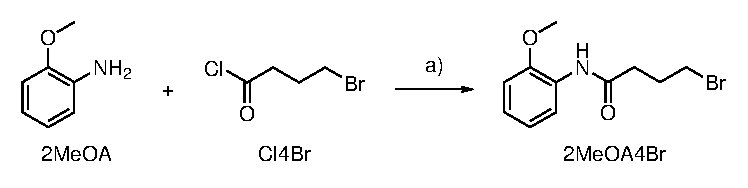
\includegraphics[scale=1]{2MeOA4Br_synth}
		\caption{Synthesis of Br-C$_4$-2-methoxybenzene \compound{cmpd:2MeOA4Br}.
		a) \ce{NaHCO3}, \ce{CH2Cl2}, \ce{H2O}, 0 $^{\circ}$C, 1 h, 50.0 \%.
		\label{sch:2MeOA4Br_synth}}
	\end{center}
\end{scheme}

The procedure outlined by Ganguly \textit{et al.}\cite{Ganguly2011} was initially attempted in order to synthesise the 2-methoxybenzene-CipMe conjugate \compound{cmpd:2MeOA4CipMe}, but the reaction was very slow and did not go to completion, presumably due to degradation of Br-C$_4$-2-methoxybenzene \compound{cmpd:2MeOA4Br}.
New conditions, employing a microwave reactor and 2 eq. of Br-C$_4$-2-methoxybenzene \compound{cmpd:2MeOA4Br} were then attempted, with a much greater conversion observed by LCMS after 4 h. However, a poor yield was obtained, potentially due to degradation during column chromatography, which took longer than for Br-C$_4$-2-methoxybenzene \compound{cmpd:2MeOA4Br} because the 2-methoxybenzene-CipMe conjugate \compound{cmpd:2MeOA4CipMe} is more polar.

\ce{N3}-C$_4$-2-methoxybenzene \compound{cmpd:2MeOA4N3} was synthesised from Br-C$_4$-2-methoxybenzene \compound{cmpd:2MeOA4Br} by an S$_N$2 reaction with sodium azide. The yield of \ce{N3}-C$_4$-2-methoxybenzene \compound{cmpd:2MeOA4N3} (26.7 \%) was a lot lower than for \ce{N3}-C$_4$-HCTL \compound{cmpd:SHL4N3} (89.3 \%). The colour of \ce{N3}-C$_4$-2-methoxybenzene \compound{cmpd:2MeOA4N3}, like its precursor, changed from clear to blue then black, suggesting that it is also air/light sensitive and may have degraded during columning. However, in this case it may not be better to use this product crude as several impurities could be observed by LCMS (see \ref{fig:2MeOA4N3_impurities}).

\begin{scheme}[H]
	\begin{center}
		\schemeref[2MeOA4Br]{cmpd:2MeOA4Br}
		\schemeref[CipMe]{cmpd:CipMe}
		\schemeref[2MeOA4CipMe]{cmpd:2MeOA4CipMe}	
		\schemeref[2MeOA4N3]{cmpd:2MeOA4N3}
		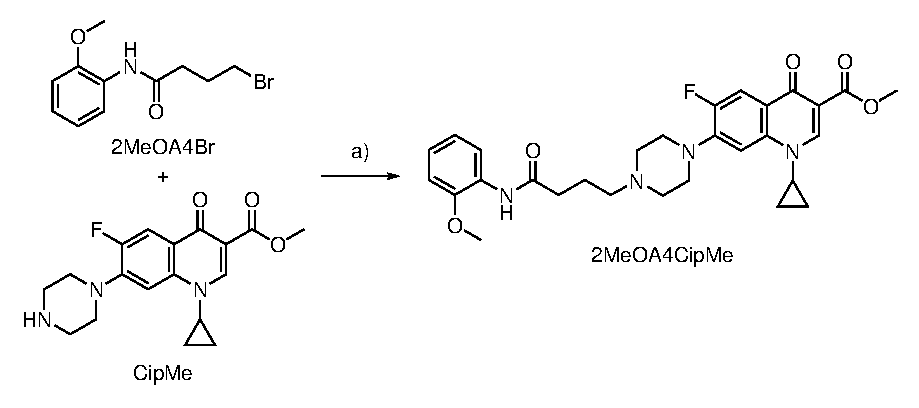
\includegraphics[scale=1]{2MeOA4_synth}
		\caption{Synthesis of the 2-methoxybenzene-CipMe conjugate \compound{cmpd:2MeOA4CipMe} and \ce{N3}-C$_4$-2-methoxybenzene \compound{cmpd:2MeOA4N3}. 
		a)  DIPEA, \ce{NaI}, acetonitrile, microwave reactor, 100 $^{\circ}$C, 4 h, 10.2 \%.
		b) \ce{NaN3}, acetonitrile, reflux, 2 h, 26.7 \%.  \label{sch:2MeOA4_synth}}
	\end{center}
\end{scheme}


\begin{figure}[H]
	\begin{center}
		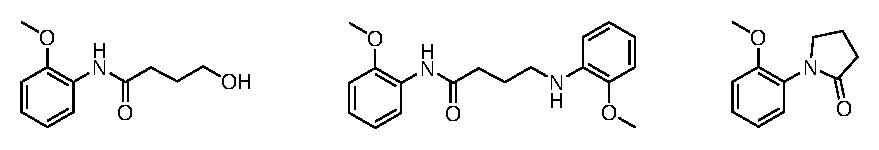
\includegraphics[scale=1]{2MeOA4N3_impurities}
		\caption{Impurities formed during the synthesis of \ce{N3}-C$_4$-2-methoxybenzene \compound{cmpd:2MeOA4N3}.
		\label{fig:2MeOA4N3_impurities}}
	\end{center}
\end{figure}

ditto

\begin{scheme}[H]
	\begin{center}
		\schemeref[2MeOA4N3]{cmpd:2MeOA4N3}
		\schemeref[Y4Cip]{cmpd:Y4Cip}
		\schemeref[2MeOA4T4Cip]{cmpd:2MeOA4T4Cip}		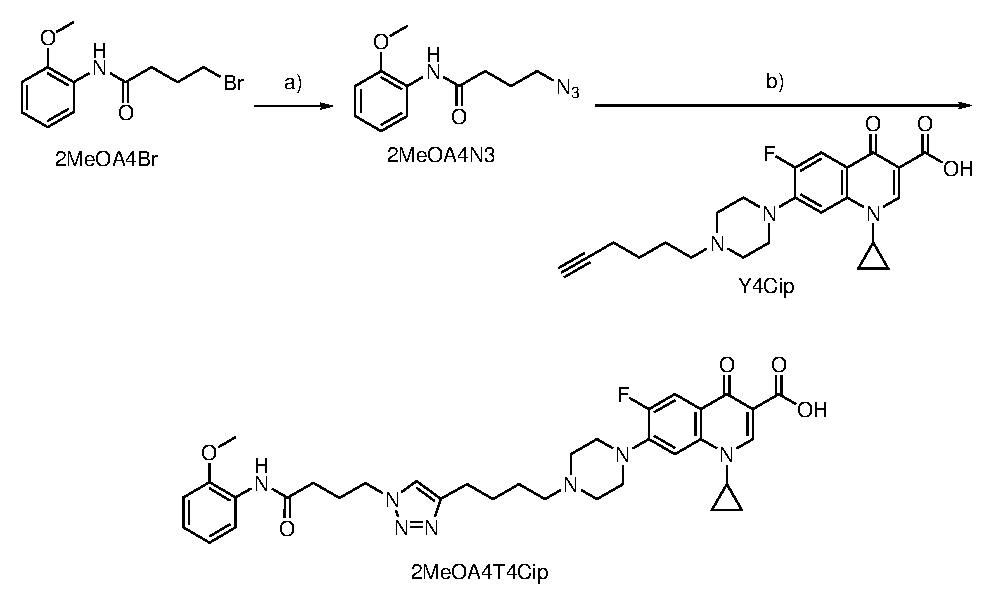
\includegraphics[scale=1]{2MeOA4T4Cip_synth}
		\caption{Synthesis of the 2-methoxybenzene-Cip triazole conjugate \compound{cmpd:2MeOA4T4Cip}. 
		a) \ce{CuSO4}, THPTA, sodium ascorbate, \ce{H2O}, \textit{t}-BuOH, \ce{CH2Cl2}, r.t., 16 h, 39.0 \%.\label{sch:2MeOA4T4Cip_synth}}
	\end{center}
\end{scheme}

\subsection{Synthesis of the 3-methoxyphenyl derivatives}

\begin{scheme}[H]
	\begin{center}
		\schemeref[3MeOA]{cmpd:3MeOA}
		\schemeref[Cl4Br]{cmpd:Cl4Br}
		\schemeref[3MeOA4Br]{cmpd:3MeOA4Br}
		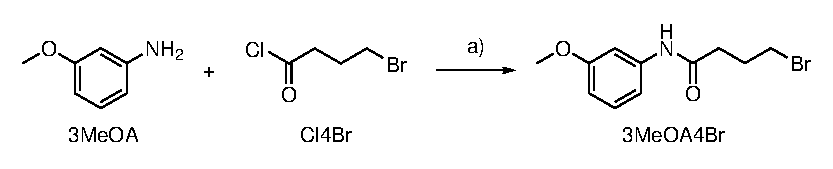
\includegraphics[scale=1]{3MeOA4Br_synth}
		\caption{Synthesis of Br-C$_4$-3-methoxybenzene \compound{cmpd:2MeOA4Br}.
				a) \ce{NaHCO3}, \ce{CH2Cl2}, \ce{H2O}, 0 $^{\circ}$C, 1 h, 49.6 \%. \label{sch:3MeOA4Br_synth}}
	\end{center}
\end{scheme}

\begin{scheme}[H]
	\begin{center}
		\schemeref[3MeOA4Br]{cmpd:3MeOA4Br}
		\schemeref[CipMe]{cmpd:CipMe}
		\schemeref[3MeOA4CipMe]{cmpd:3MeOA4CipMe}	
		\schemeref[3MeOA4N3]{cmpd:3MeOA4N3}
		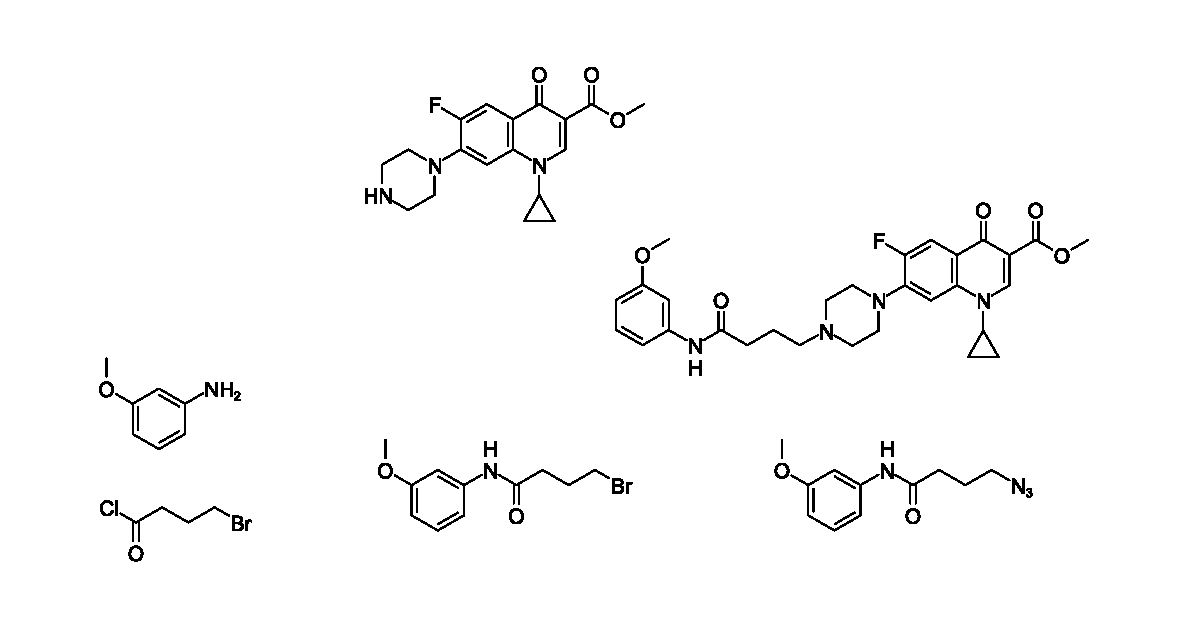
\includegraphics[scale=1]{3MeOA4_synth}
		\caption{Synthesis of the 3-methoxybenzene-CipMe conjugate \compound{cmpd:3MeOA4CipMe} and \ce{N3}-C$_4$-3-methoxybenzene \compound{cmpd:3MeOA4N3}. 
				a)  DIPEA, \ce{NaI}, acetonitrile, microwave reactor, 100 $^{\circ}$C, 4 h, 10.5 \%.
				b) \ce{NaN3}, acetonitrile, reflux, 7 h, 16.7 \%.  \label{sch:3MeOA4_synth}}
	\end{center}
\end{scheme}

\begin{scheme}[H]
	\begin{center}
		\schemeref[3MeOA4N3]{cmpd:3MeOA4N3}
		\schemeref[Y4Cip]{cmpd:Y4Cip}
		\schemeref[3MeOA4T4Cip]{cmpd:3MeOA4T4Cip}		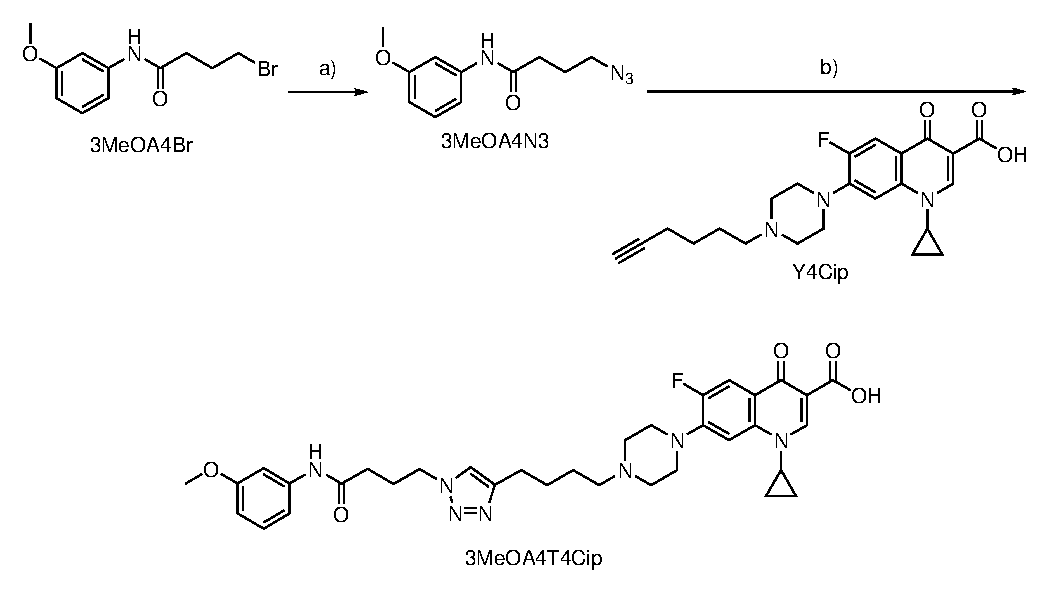
\includegraphics[scale=1]{3MeOA4T4Cip_synth}
		\caption{Synthesis of the 3-methoxybenzene-Cip triazole conjugate \compound{cmpd:3MeOA4T4Cip}. 
				a) \ce{CuSO4}, THPTA, sodium ascorbate, \ce{H2O}, \textit{t}-BuOH, \ce{CH2Cl2}, r.t., 2 h, 5.0 \%. \label{sch:3MeOA4T4Cip_synth}}
	\end{center}
\end{scheme}

